\chapter{Árvores Vermelho-Preto}

Árvores balanceadas são estruturas fundamentais para garantir eficiência em operações de busca, inserção e remoção em tempo logarítmico. 
No capítulo anterior, estudamos as árvores B, voltadas principalmente para sistemas de armazenamento externo, como bancos de dados e sistemas de arquivos. 
Antes delas, vimos as árvores AVL, que mantêm um balanceamento rigoroso por meio de diferenças de altura entre subárvores.

As árvores vermelho-preto oferecem uma abordagem diferente: relaxam o critério de balanceamento das AVL em troca de algoritmos mais simples e eficientes para inserção e remoção. 
Em vez de controlar diferenças de altura, usam uma coloração (vermelha ou preta) em cada nó, junto a regras que garantem que a altura da árvore permaneça proporcional a $\log n$. 

Neste capítulo, estudaremos as propriedades que definem as árvores vermelho-preto, os algoritmos de inserção e remoção que mantêm essas propriedades.

Uma \textbf{árvore vermelho-preto} é uma árvore binária de busca em que cada nó contém, além da chave, uma \textbf{cor}: vermelha ou preta. 
O balanceamento da árvore é garantido por um conjunto de propriedades que limitam a forma como os nós vermelhos e pretos podem ser organizados. 
Essas regras asseguram que a altura da árvore permaneça proporcional a $\log n$.

As cinco propriedades fundamentais de uma árvore vermelho-preto são:

\begin{enumerate}
    \item \textbf{Cada nó é vermelho ou preto.} \\
    A cor é um atributo armazenado em cada nó da árvore.

    \item \textbf{A raiz é sempre preta.} \\
    Essa regra é aplicada após cada operação que altera a árvore.

    \item \textbf{Todas as folhas (nós nulos) são pretas.} \\
    Consideramos que todas as referências nulas -- ou seja, os ponteiros para filhos inexistentes -- são nós pretos.

    \item \textbf{Um nó vermelho não pode ter filhos vermelhos.} \\
    Ou seja, dois nós vermelhos nunca aparecem consecutivamente em um caminho.

    \item \textbf{Todos os caminhos de um nó até qualquer folha descendente contêm o mesmo número de nós pretos.} \\
    Esse número é chamado de \textit{altura preta} do nó.
\end{enumerate}

Essas propriedades impõem uma estrutura que impede o crescimento exagerado da altura, mesmo sem exigir um balanceamento rígido como nas árvores AVL.

\subsection*{Exemplo}

A figura abaixo ilustra uma árvore vermelho-preto que satisfaz todas as propriedades:

\begin{center}
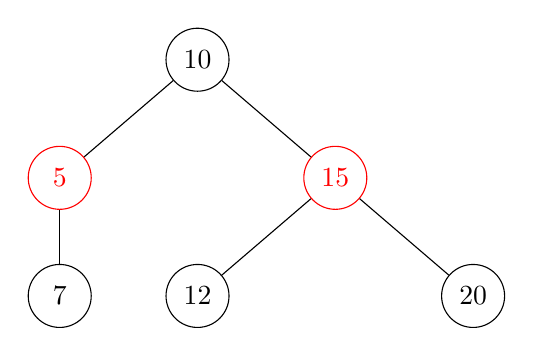
\begin{tikzpicture}[
    every node/.style={draw, circle, minimum size=8mm, inner sep=0pt},
    level distance=1.5cm, sibling distance=3.5cm
]
\tikzset{
    preto/.style={draw=black},
    vermelho/.style={draw=red, text=red}
}
\node[preto] {10}
    child {
        node[vermelho] {5}
        child[grow=down] { node[preto] {7} }
    }
    child {
        node[vermelho] {15}
        child { node[preto] {12} }
        child { node[preto] {20} }
    };
\end{tikzpicture}
\end{center}


As propriedades das árvores vermelho-preto impõem restrições que evitam o crescimento descontrolado da altura da árvore, mesmo sem exigir um balanceamento tão rigoroso quanto o das árvores AVL. 
O segredo está em como as cores limitam a estrutura dos caminhos da raiz até as folhas.

A chave da análise está na \textbf{altura preta}, definida como o número de nós pretos em qualquer caminho da raiz até uma folha. 
Pela propriedade (5), todos esses caminhos têm a mesma altura preta, digamos $bh(x)$ para um nó $x$. 
Isso significa que os caminhos não podem variar muito em comprimento: se um caminho tivesse muitos nós vermelhos consecutivos, violaria a propriedade (4), que proíbe dois vermelhos seguidos. 
Assim, o número de nós vermelhos em qualquer caminho é no máximo igual ao número de nós pretos.

Logo, o \textbf{comprimento máximo de qualquer caminho} da raiz até uma folha é no máximo o dobro da altura preta. 
Isso implica:

\[
\text{altura da árvore } \leq 2 \cdot bh(\text{raiz})
\]

Além disso, o número mínimo de nós em uma árvore com altura preta $bh$ ocorre quando todos os nós pretos estão intercalados com vermelhos, ou seja, com altura total $2 \cdot bh$. 
Mostra-se por indução que uma árvore vermelho-preto com $n$ nós tem altura no máximo:

\[
\text{altura} \leq 2 \log(n + 1)
\]

Isso garante que todas as operações de inserção, remoção e busca, que percorrem a árvore do topo até uma folha, têm custo assintótico de $O(\log n)$ no pior caso, mantendo a eficiência da estrutura mesmo após várias atualizações.


\section{Relação com as Árvores 2-3}

Uma maneira elegante de compreender as árvores vermelho-preto é enxergá-las como uma representação binária das \textbf{árvores 2-3}.
Essa correspondência, proposta por Robert Sedgewick, revela que as propriedades das árvores vermelho-preto são equivalentes às das árvores 2-3 e explica por que elas mantêm o balanceamento de forma natural.

\subsection*{Árvores 2-3}

Uma árvore 2-3 é uma árvore de busca balanceada em que cada nó pode conter uma ou duas chaves:
\begin{itemize}
\item Um \textbf{2-nó} contém uma única chave e dois filhos (à esquerda e à direita).
\item Um \textbf{3-nó} contém duas chaves e três filhos (à esquerda, ao centro e à direita).
\end{itemize}

Todas as folhas de uma árvore 2-3 estão no mesmo nível, o que garante que sua altura seja sempre proporcional a $\log n$.
A ideia central das árvores vermelho-preto é simular essa mesma estrutura usando apenas ponteiros binários.

\subsection*{Correspondência entre 2-3 e Vermelho-Preto}

A correspondência entre as duas estruturas é simples:

\begin{itemize}
\item Cada \textbf{2-nó} de uma árvore 2-3 é representado por um nó \textbf{preto} isolado em uma árvore vermelho-preto.
\item Cada \textbf{3-nó} é representado por dois nós conectados por um \textbf{link vermelho inclinado à esquerda}.
\end{itemize}

Em outras palavras, o \textbf{link vermelho} une duas chaves que pertenciam ao mesmo nó da árvore 2-3.
Os \textbf{links pretos} representam conexões entre nós distintos da árvore 2-3.

\begin{center}
\renewcommand{\arraystretch}{1.5}
\[
\begin{array}{ccc}
\textbf{Árvore 2-3} & & \textbf{Árvore vermelho-preto} \\[6pt]

\begin{array}{ccccccc}
  \boxed{c_0} & k_1 = 10 & \boxed{c_1} & k_2 = 20 & \boxed{c_2} \\
  \downarrow  &           & \downarrow  &          & \downarrow  \\
  <10 &
  &
  10{\,<\,}x{\,<\,}20 &
  &
  >20
\end{array}
&\qquad&
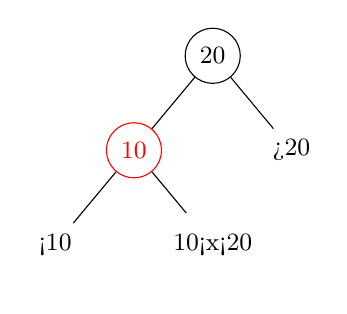
\begin{tikzpicture}[level distance=1.2cm,
  every node/.style={circle, minimum size=7mm, inner sep=0pt, font=\small},
  sibling distance=2cm
]
\tikzset{
  preto/.style={draw=black},
  vermelho/.style={draw=red, text=red}
}

\node[preto] (a) {20}
  child {
    node[vermelho] {10}
      child {node {<10}}
      child {node {10<x<20}}
  }
  child {node {>20}};
\end{tikzpicture}
\end{array}
\]
\end{center}


Nessa codificação, cada \textbf{link vermelho à esquerda} representa a fusão de dois nós consecutivos da árvore binária em um único 3-nó da árvore 2-3.
Por convenção, as árvores vermelho-preto são implementadas com links vermelhos sempre inclinados à esquerda — isso evita ambiguidade e simplifica os algoritmos.

\subsection*{Equivalência estrutural}

Essa correspondência garante que:
\begin{itemize}
\item Não existem dois links vermelhos consecutivos — o que equivaleria a um nó 4 em uma árvore 2-3, proibido por definição.
\item Todo caminho da raiz até uma folha contém o mesmo número de links pretos — o que corresponde à propriedade de que todas as folhas de uma árvore 2-3 estão na mesma profundidade.
\end{itemize}

Assim, cada árvore vermelho-preto é uma árvore binária de busca que mantém exatamente as mesmas restrições estruturais de uma árvore 2-3, mas representadas por cores em vez de múltiplas chaves por nó.

\subsection*{Implicações práticas}

Ver as árvores vermelho-preto como codificações de árvores 2-3 tem duas vantagens conceituais importantes:
\begin{enumerate}
\item Permite compreender suas operações (inserção e remoção) como transformações locais que preservam a equivalência com a árvore 2-3.
\item Explica por que a altura das árvores vermelho-preto está limitada por $2 \log (n + 1)$: é a altura de uma árvore 2-3 “expandida” em forma binária.
\end{enumerate}

Em outras palavras, as árvores vermelho-preto combinam a \textbf{estrutura balanceada} das árvores 2-3 com a \textbf{simplicidade} das árvores binárias de busca.
Essa visão servirá de base para entender as operações de inserção e remoção que estudaremos a seguir.


\section{Função {\tt inserir}}

\section{Inserção}

A inserção em uma árvore vermelho-preto segue duas etapas principais:

\begin{enumerate}
    \item Inserir o novo nó como em uma árvore binária de busca (ABB) comum.
    \item Colorir o novo nó como \textbf{vermelho} e, em seguida, executar uma sequência de \textbf{recolorações} e possivelmente \textbf{rotações} para restaurar as propriedades vermelho-preto.
\end{enumerate}

Colorir o novo nó de vermelho ajuda a manter a propriedade (5) (altura preta), mas pode violar a propriedade (4) (nenhum nó vermelho pode ter filho vermelho). Para resolver essa violação, aplicamos um procedimento de correção que depende da cor do \textit{tio} do novo nó.

\subsection*{Leitura da inserção via árvores 2-3}

Como vimos, uma árvore vermelho-preto pode ser interpretada como uma codificação binária de uma árvore 2-3 (links vermelhos representam a fusão local que forma um 3-nó). Nessa visão, cada passo da inserção RB corresponde a uma operação natural em 2-3:

\begin{enumerate}
  \item \textbf{Inserir como ABB} $\Rightarrow$ \textbf{descer até a folha na 2-3} e tentar acomodar a nova chave no nó corrente (um 2-nó vira 3-nó; um 3-nó pode “estourar”).
  \item \textbf{Colorir de vermelho} $\Rightarrow$ \textbf{juntar a chave ao nó 2-3 corrente}, isto é, representar um 3-nó por um link vermelho.
  \item \textbf{Recolorar/rotacionar} $\Rightarrow$ \textbf{corrigir estouros (split) e promover a mediana}, quando um nó temporário com três chaves (nó~4) aparece.
\end{enumerate}

\noindent\textbf{Tradução caso a caso.}
Ao tratar a violação ``pai vermelho'', inspecionamos a cor do tio (na RB); na 2-3, isso indica se há \emph{split} ou apenas recodificação local:

\begin{center}
\renewcommand{\arraystretch}{1.2}
\begin{tabularx}{\linewidth}{@{}>{\bfseries}l >{\raggedright\arraybackslash}X >{\raggedright\arraybackslash}X@{}}
\toprule
Caso RB & Ação na RB & Leitura em 2-3 \\
\midrule
1. Tio vermelho & Flip de cores (pai/tio $\to$ preto; avô $\to$ vermelho) &
\emph{Split} de nó 4: mediana sobe; pode propagar para cima. \\
2. Tio preto, zig-zag & Rotação simples para “endireitar” &
Só recodificação: 3-nó permanece o mesmo, forma canônica. \\
3. Tio preto, em linha & Rotação + flip de cores &
\emph{Split} local: mediana torna-se pai; filhos viram 2-nós. \\
\bottomrule
\end{tabularx}
\end{center}

\noindent\textbf{Mnemônico.}
\[
\underbrace{\text{flip de cores}}_{\text{RB}}
\;\Longleftrightarrow\;
\underbrace{\text{split de nó 4}}_{\text{2-3}}
\qquad\text{e}\qquad
\underbrace{\text{rotação}}_{\text{RB}}
\;\Longleftrightarrow\;
\underbrace{\text{reorientar / elevar a mediana}}_{\text{2-3}}.
\]

\medskip

Os principais casos de rebalanceamento são:

\begin{itemize}

\item \textbf{Caso 1 (Tio vermelho):} recolorimos pai, tio e avô.

Esse caso corresponde, na árvore 2-3, à situação em que a inserção gera temporariamente um \textbf{nó 4}, ou seja, um nó com três chaves \texttt{(B, A, C)}.  
A recoloração na árvore vermelho-preto equivale a dividir esse nó 4 em três nós 2 separados, promovendo a chave do meio (\texttt{A}) para o nível acima.

\begin{center}
\renewcommand{\arraystretch}{1.5}
\[
\begin{array}{ccc}
\textbf{Árvore 2-3} & & \textbf{Árvore vermelho-preto} \\[6pt]

\begin{array}{cccccccc}
  \boxed{}    & k_1 = B & \boxed{}    & k_2 = A & \boxed{}    & k_3 = C & \boxed{} \\
  \downarrow  &         & \downarrow  &         & \downarrow  &         & \downarrow  \\
              &         & [N]         &         &             &         &             \\
\end{array}

&\qquad&
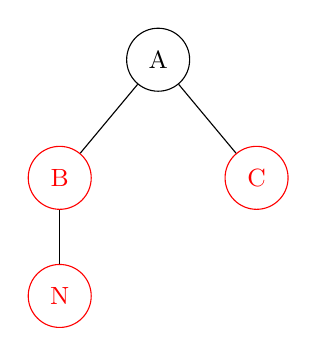
\begin{tikzpicture}[
  every node/.style={draw, circle, minimum size=8mm, inner sep=0pt, font=\small},
  level distance=1.5cm, sibling distance=2.5cm
]
\tikzset{
  preto/.style={draw=black},
  vermelho/.style={draw=red, text=red}
}
\node[preto] {A}
  child {
    node[vermelho] {B}
      child[grow=down] { node[vermelho] {N} } % novo nó inserido
  }
  child { node[vermelho] {C} };
\end{tikzpicture}
\end{array}
\]
\end{center}

Após a recoloração, a chave \texttt{A} é promovida e as chaves \texttt{B} e \texttt{C} se tornam nós pretos independentes.  
Na árvore 2-3, isso corresponde à divisão do nó 4 em três nós 2, mantendo o balanceamento da altura.

\begin{center}
\renewcommand{\arraystretch}{1.5}
\[
\begin{array}{ccc}
\textbf{Árvore 2-3} & & \textbf{Árvore vermelho-preto} \\[6pt]

\begin{array}{ccc}
  \boxed{}           & k_1 = A & \boxed{} \\
  \downarrow         &         & \downarrow      \\
  \text{[B,  N]}     &         & [C]       \\
\end{array}


&\qquad&
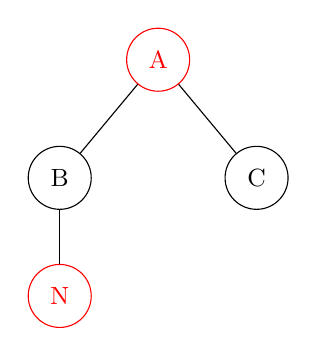
\begin{tikzpicture}[
  every node/.style={draw, circle, minimum size=8mm, inner sep=0pt, font=\small},
  level distance=1.5cm, sibling distance=2.5cm
]
\tikzset{
  preto/.style={draw=black},
  vermelho/.style={draw=red, text=red}
}
\node[vermelho] {A}
  child {
    node[preto] {B}
      child[grow=down] { node[vermelho] {N} }
  }
  child { node[preto] {C} };
\end{tikzpicture}
\end{array}
\]
\end{center}


\item \textbf{Caso 2 (Tio preto e filho em zig-zag):} rotação simples para transformar em Caso 3.

\begin{center}
\renewcommand{\arraystretch}{1.5}
\[
\begin{array}{ccc}
\textbf{Árvore 2-3} & & \textbf{Árvore vermelho-preto} \\[6pt]

\begin{array}{ccc}
  \boxed{} \;     & k_1 = A & \; \boxed{} \\
  \downarrow      &         &   \downarrow   \\
  \text{[C]}      &         & \text{[N, B]} \\
\end{array}
&\qquad&
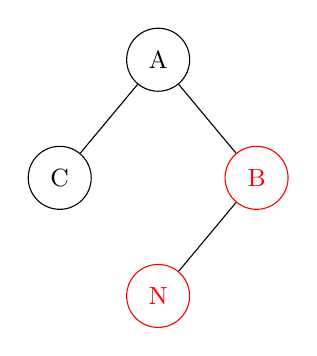
\begin{tikzpicture}[
  every node/.style={draw, circle, minimum size=8mm, inner sep=0pt, font=\small},
  level distance=1.5cm, sibling distance=2.5cm
]
\tikzset{
  preto/.style={draw=black},
  vermelho/.style={draw=red, text=red}
}
\node[preto] {A}
  child { node[preto] {C} }
  child {
    node[vermelho] {B}
      child { node[vermelho] {N} } % N é filho à esquerda de B → zig-zag
      child[missing]
  };
\end{tikzpicture}
\end{array}
\]
\end{center}

\noindent
\emph{Interpretação 2-3:} o filho direito de \([A]\) é um \textbf{3-nó} \([\;N,\;B\;]\).  
Na vermelho-preto, porém, esse 3-nó está codificado com um \textbf{link vermelho torto} (direita-depois-esquerda): é o “zig-zag”.

\medskip

\begin{center}
\renewcommand{\arraystretch}{1.5}
\[
\begin{array}{ccc}
\textbf{Árvore 2-3} & & \textbf{Árvore vermelho-preto} \\[6pt]

\begin{array}{ccc}
  \boxed{} \;     & k_1 = A & \; \boxed{} \\
  \downarrow      &         &   \downarrow   \\
  \text{[C]}      &         & \text{[N, B]} \\
\end{array}
&\qquad&
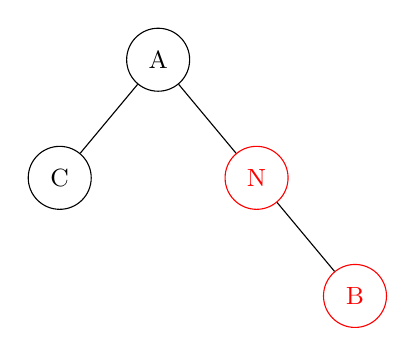
\begin{tikzpicture}[
  every node/.style={draw, circle, minimum size=8mm, inner sep=0pt, font=\small},
  level distance=1.5cm, sibling distance=2.5cm
]
\tikzset{
  preto/.style={draw=black},
  vermelho/.style={draw=red, text=red}
}
\node[preto] {A}
  child { node[preto] {C} }
  child {
    node[vermelho] {N}
      child[missing]
      child { node[vermelho] {B} } % agora é “em linha” (equivalente ao Caso 3)
  };
\end{tikzpicture}
\end{array}
\]
\end{center}


\item \textbf{Caso 3 (Tio preto e filho em linha):} rotação e recoloração.

\begin{center}
\renewcommand{\arraystretch}{1.5}
\[
\begin{array}{ccc}
\textbf{Árvore 2-3} & & \textbf{Árvore vermelho-preto} \\[6pt]

\begin{array}{ccc}
  \boxed{} \; & k_1 = A & \; \boxed{}  \\
  \downarrow  &         &   \downarrow \\
  C           &         & B, N         \\
\end{array}
&\qquad&
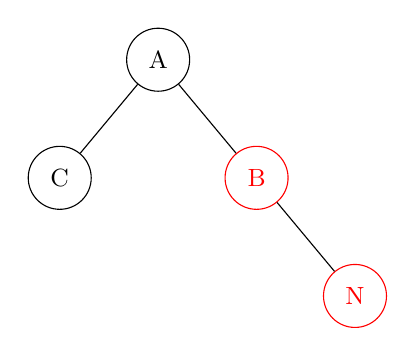
\begin{tikzpicture}[
  every node/.style={draw, circle, minimum size=8mm, inner sep=0pt, font=\small},
  level distance=1.5cm, sibling distance=2.5cm
]
\tikzset{
  preto/.style={draw=black},
  vermelho/.style={draw=red, text=red}
}
\node[preto] {A}
  child { node[preto] {C} }
  child {
    node[vermelho] {B}
      child[missing]
      child { node[vermelho] {N} } % em linha (direita-depois-direita)
  };
\end{tikzpicture}
\end{array}
\]
\end{center}

\noindent
\emph{Leitura 2-3:} o filho direito de \([A]\) é o \textbf{3-nó} \([B,N]\) (com \(B < N\)).  
Na vermelho-preto, corrigimos a codificação (link vermelho à direita e vermelho duplo) com \textbf{rotação à esquerda em \(A\)} seguida de \textbf{troca de cores}.

\medskip

\begin{center}
\renewcommand{\arraystretch}{1.5}
\[
\begin{array}{ccc}
\textbf{Árvore 2-3} & & \textbf{Árvore vermelho-preto} \\[6pt]

\begin{array}{ccc}
  \boxed{\ [A]\ } & \; k_1 = B \; & \boxed{\ [N]\ } \\
  \downarrow      &               & \downarrow      \\
  C               &               &                 \\  
\end{array}
&\qquad&
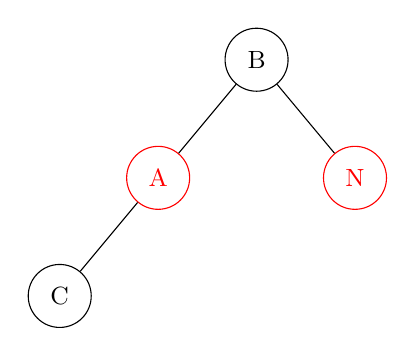
\begin{tikzpicture}[
  every node/.style={draw, circle, minimum size=8mm, inner sep=0pt, font=\small},
  level distance=1.5cm, sibling distance=2.5cm
]
\tikzset{
  preto/.style={draw=black},
  vermelho/.style={draw=red, text=red}
}
\node[preto] {B}
  child {
    node[vermelho] {A}
      child { node[preto] {C} }
      child[missing]
  }
  child { node[vermelho] {N} };
\end{tikzpicture}
\end{array}
\]
\end{center}


\end{itemize}


A seguir, um esboço da função de inserção com chamada à função de correção:

\begin{lstlisting}[language=C, caption={Inserção em árvore vermelho-preto (esboço)}, label=lst:insercao_rb]
typedef enum { VERMELHO, PRETO } Cor;

typedef struct No {
    int chave;
    Cor cor;
    struct No *esq, *dir, *pai;
} No;

void inserir(No **raiz, int chave) {
    No *novo = criar_no(chave, VERMELHO);
    inserir_abb(raiz, novo);
    corrigir_insercao(raiz, novo);
}
\end{lstlisting}

A função \texttt{corrigir\_insercao} é responsável por garantir que as propriedades da árvore vermelho-preto sejam restauradas após a inserção.

\begin{lstlisting}[language=C, caption={Correção após inserção em árvore vermelho-preto}, label=lst:corrigir_insercao]
void corrigir_insercao(No **raiz, No *n) {
    while (n != *raiz && n->pai->cor == VERMELHO) {
        No *pai = n->pai;
        No *avo = pai->pai;

        if (pai == avo->esq) {
            No *tio = avo->dir;

            if (tio && tio->cor == VERMELHO) {
                // Caso 1: tio vermelho
                pai->cor = PRETO;
                tio->cor = PRETO;
                avo->cor = VERMELHO;
                n = avo; // sobe para verificar novo conflito
            } else {
                if (n == pai->dir) {
                    // Caso 2: zig-zag
                    n = pai;
                    rotacao_esquerda(raiz, n);
                }
                // Caso 3: linha reta
                pai = n->pai;
                avo = pai->pai;
                pai->cor = PRETO;
                avo->cor = VERMELHO;
                rotacao_direita(raiz, avo);
            }
        } else {
            // simétrico: pai está à direita
            No *tio = avo->esq;

            if (tio && tio->cor == VERMELHO) {
                // Caso 1 (simétrico)
                pai->cor = PRETO;
                tio->cor = PRETO;
                avo->cor = VERMELHO;
                n = avo;
            } else {
                if (n == pai->esq) {
                    // Caso 2 (simétrico)
                    n = pai;
                    rotacao_direita(raiz, n);
                }
                // Caso 3 (simétrico)
                pai = n->pai;
                avo = pai->pai;
                pai->cor = PRETO;
                avo->cor = VERMELHO;
                rotacao_esquerda(raiz, avo);
            }
        }
    }

    (*raiz)->cor = PRETO;
}
\end{lstlisting}

\section{Função {\tt remover}}

A operação de remoção em árvores vermelho-preto segue a mesma ideia geral da remoção em árvores binárias de busca (ABB):

\begin{enumerate}
    \item Localizamos o nó a ser removido.
    \item Se ele tiver dois filhos, substituímos seu valor pelo de seu sucessor imediato (ou antecessor) e então removemos esse sucessor, que terá no máximo um filho.
    \item O nó removido de fato terá, portanto, no máximo um filho (como em uma ABB).
\end{enumerate}

No entanto, como as cores dos nós afetam diretamente as propriedades da árvore, a remoção pode gerar violações nas propriedades vermelho-preto, principalmente a da altura preta. 
Isso acontece especialmente quando se remove um nó preto.

Para lidar com essas violações, introduzimos o conceito de {\em nó duplamente preto}, que aparece temporariamente durante o processo de correção. 
Ele representa um déficit de cor e será tratado com rotações e recolorações, até que todas as propriedades sejam restauradas.

Abaixo está um esboço da função de remoção, com chamada a uma função de correção:

\begin{lstlisting}[language=C, caption={Remoção em árvore vermelho-preto}, label=lst:remocao_rb]
void remover(No **raiz, int chave) {
    No *n = buscar(*raiz, chave);
    if (n == NULL) return;

    No *substituto = n;
    Cor cor_original = substituto->cor;

    No *x; // nó que sobe (pode ser nulo)

    if (n->esq == NULL) {
        x = n->dir;
        transplantar(raiz, n, n->dir);
    } else if (n->dir == NULL) {
        x = n->esq;
        transplantar(raiz, n, n->esq);
    } else {
        substituto = minimo(n->dir);
        cor_original = substituto->cor;
        x = substituto->dir;

        if (substituto->pai == n) {
            if (x) x->pai = substituto;
        } else {
            transplantar(raiz, substituto, substituto->dir);
            substituto->dir = n->dir;
            substituto->dir->pai = substituto;
        }

        transplantar(raiz, n, substituto);
        substituto->esq = n->esq;
        substituto->esq->pai = substituto;
        substituto->cor = n->cor;
    }

    if (cor_original == PRETO)
        corrigir_remocao(raiz, x);
}
\end{lstlisting}

A função auxiliar \texttt{corrigir\_remocao} é responsável por eliminar o nó duplamente preto que pode surgir após a remoção de um nó preto.

Durante a correção, tratamos uma série de casos que dependem da cor do irmão do nó duplamente preto e de seus filhos:

\begin{itemize}
    \item \textbf{Caso 1:} irmão vermelho
	\begin{center}
		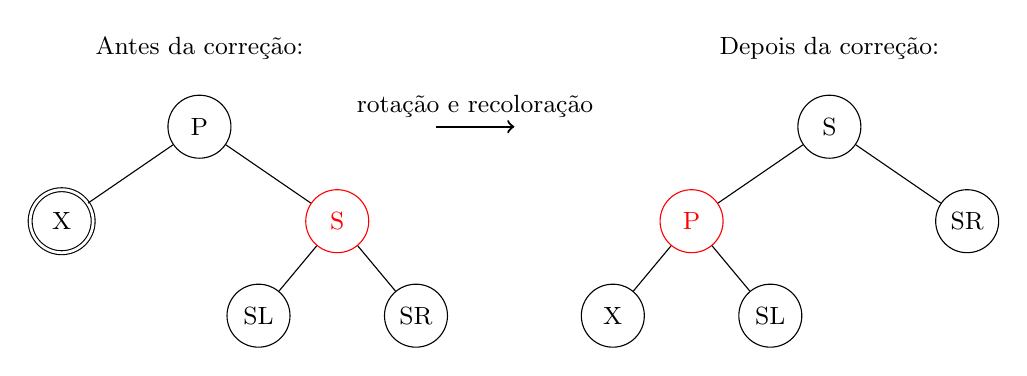
\begin{tikzpicture}[
		  level distance=1.2cm,
		  level 1/.style={sibling distance=3.5cm},
		  level 2/.style={sibling distance=2cm},
		  every node/.style={font=\small}
		]

		\tikzset{
		    preto/.style={draw=black, circle, minimum size=8mm, inner sep=1pt},
		    vermelho/.style={draw=red, text=red, draw=red, circle, minimum size=8mm, inner sep=1pt},
		    duplo/.style={draw=black, double distance=1pt, circle, minimum size=8mm, inner sep=1pt}
		}

		% Antes da correção
		\node at (-5,0) {Antes da correção:};

		\node[preto] (P) at (-5,-1) {P}
		  child { node[duplo] {X} }
		  child { node[vermelho] (S) {S}
		    child { node[preto] {SL} }
		    child { node[preto] {SR} }
		  };

		% Seta de transformação
		\draw[->, thick] (-2,-1) -- (-1,-1) node[midway, above] {rotação e recoloração};

		% Depois da correção
		\node at (3,0) {Depois da correção:};

		\node[preto] (S2) at (3,-1) {S}
		  child { node[vermelho] (P2) {P}
		    child { node[preto] {X} }
		    child { node[preto] {SL} }
		  }
		  child { node[preto] {SR} };

		\end{tikzpicture}
	\end{center}




    \item \textbf{Caso 2:} irmão preto com filhos pretos

	\begin{center}
		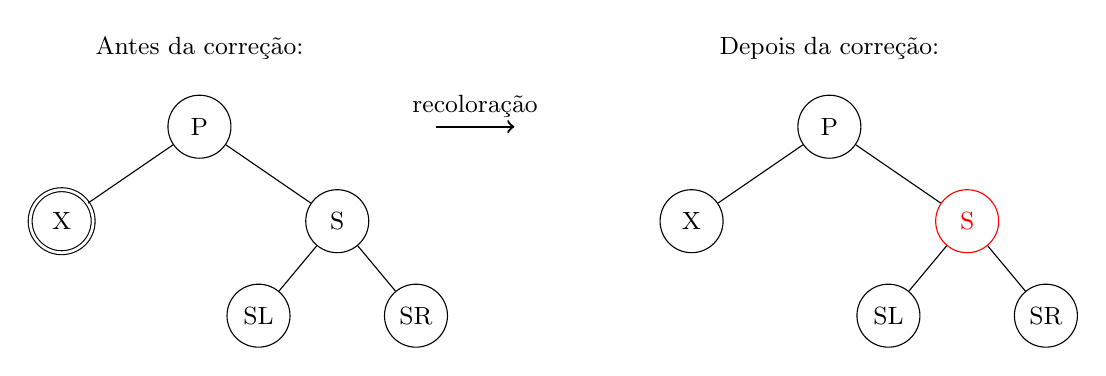
\begin{tikzpicture}[
		  level distance=1.2cm,
		  level 1/.style={sibling distance=3.5cm},
		  level 2/.style={sibling distance=2cm},
		  every node/.style={font=\small}
		]

		\tikzset{
		    preto/.style={draw=black, circle, minimum size=8mm, inner sep=1pt},
		    vermelho/.style={draw=red, text=red, draw=red, circle, minimum size=8mm, inner sep=1pt},
		    duplo/.style={draw=black, double distance=1pt, circle, minimum size=8mm, inner sep=1pt}
		}

		% Antes da correção
		\node at (-5,0) {Antes da correção:};

		\node[preto] (P) at (-5,-1) {P}
		  child { node[duplo] {X} }
		  child { node[preto] (S) {S}
		    child { node[preto] {SL} }
		    child { node[preto] {SR} }
		  };

		% Seta de transformação
		\draw[->, thick] (-2,-1) -- (-1,-1) node[midway, above] {recoloração};

		% Depois da correção
		\node at (3,0) {Depois da correção:};

		\node[preto] (P2) at (3,-1) {P}
		  child { node[preto] {X} }
		  child { node[vermelho] (S2) {S}
		    child { node[preto] {SL} }
		    child { node[preto] {SR} }
		  };

		\end{tikzpicture}
	\end{center}


    \item \textbf{Caso 3:} irmão preto com filho vermelho longe
    \begin{center}
		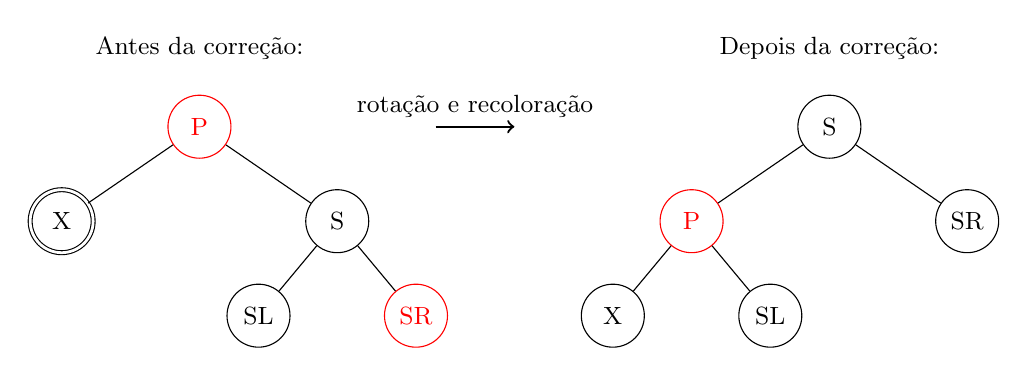
\begin{tikzpicture}[
		  level distance=1.2cm,
		  level 1/.style={sibling distance=3.5cm},
		  level 2/.style={sibling distance=2cm},
		  every node/.style={font=\small}
		]

		\tikzset{
		    preto/.style={draw=black, circle, minimum size=8mm, inner sep=1pt},
		    vermelho/.style={draw=red, text=red, draw=red, circle, minimum size=8mm, inner sep=1pt},
		    duplo/.style={draw=black, double distance=1pt, circle, minimum size=8mm, inner sep=1pt}
		}

		% Antes da correção
		\node at (-5,0) {Antes da correção:};

		\node[vermelho] (P) at (-5,-1) {P}
		  child { node[duplo] {X} }
		  child { node[preto] (S) {S}
		    child { node[preto] {SL} }
		    child { node[vermelho] {SR} }
		  };

		% seta
		\draw[->, thick] (-2,-1) -- (-1,-1) node[midway, above] {rotação e recoloração};

		% Depois da correção
		\node at (3,0) {Depois da correção:};

		\node[preto] (S2) at (3,-1) {S}
		  child {
		    node[vermelho] {P}
		    child { node[preto] {X} }
		    child { node[preto] {SL} }
		  }
		  child {
		    node[preto] {SR}
		  };

		\end{tikzpicture}
	\end{center}

    \item \textbf{Caso 4:} irmão preto com filho vermelho próximo

    \begin{center}
		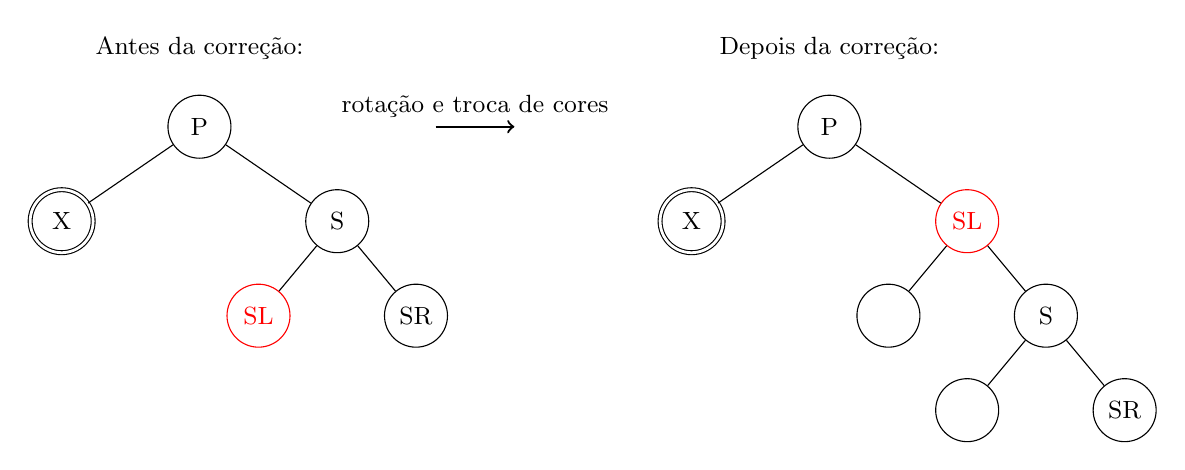
\begin{tikzpicture}[
		  level distance=1.2cm,
		  level 1/.style={sibling distance=3.5cm},
		  level 2/.style={sibling distance=2cm},
		  every node/.style={font=\small}
		]

		\tikzset{
		    preto/.style={draw=black, circle, minimum size=8mm, inner sep=1pt},
		    vermelho/.style={draw=red, text=red, draw=red, circle, minimum size=8mm, inner sep=1pt},
		    duplo/.style={draw=black, double distance=1pt, circle, minimum size=8mm, inner sep=1pt}
		}

		% Antes da correção
		\node at (-5,0) {Antes da correção:};

		\node[preto] (P) at (-5,-1) {P}
		  child { node[duplo] {X} }
		  child { node[preto] (S) {S}
		    child { node[vermelho] (SL) {SL} }
		    child { node[preto] {SR} }
		  };

		% seta
		\draw[->, thick] (-2,-1) -- (-1,-1) node[midway, above] {rotação e troca de cores};

		% Depois da correção
		\node at (3,0) {Depois da correção:};

		\node[preto] (P2) at (3,-1) {P}
		  child { node[duplo] {X} }
		  child { node[vermelho] (SL2) {SL}
		    child { node[preto] {} }
		    child { node[preto] {S}
		      child { node[preto] {} }
		      child { node[preto] {SR} }
		    }
		  };

		\end{tikzpicture}
	\end{center}

\end{itemize}

Cada um desses casos requer uma combinação específica de rotações e recolorações. 
A complexidade da remoção é maior do que a da inserção, mas a altura da árvore continua limitada por $2\log(n+1)$, e todas as operações mantêm custo assintótico de $O(\log n)$.

